\chapter{Task 1}
\begin{parlist}

\item Problem domain classes are classes used in the analysis class model to represent abstractions in the problem domain e.g. air pressure, transactions. Solution classes, on the other hand, represent abstractions in the solution domain that are introduced due to technical constraints e.g. buffer, database connection etc.

\item A problem domain class would be e.g. the class Table because databases of this kind are mainly used to store tables from the problem domain. A solution domain class would be a network connection class that controls a network connection or a database class that stores data about a database.

\item In the analysis phase class diagrams are used to model the domain, in the design phase class diagrams are used to get a shared understanding of the structure of the system within a developer team. In the implementation phase class diagrams are used to implement the system, the classes from the diagram are directly translated into code.

	%\item Application domain classes are constructed from the  domain/requirements engineering in the system analysis, or inception, phase of a development project. They are mostly solution independent in a sense that are not bound to any platform to be developed with(they are not specifically Java classes for example). Do not represent any type of methods, they are ofter depicted with responsibilities. Often application domain classes don't depict any types for their attributes. See figure \ref{fig:ADC}. \\
	%	Unlike application domain classes, solution domain classes are indeed platform dependent and need methods that translates at least partially their responsibility. Compared to the previous type, SDC can often have arrows that imprint directions and therefore more precision when depicting associations between classes. SDC also have to specify types for their attributes. See figure \ref{fig:SDC}.
	%\item In particular for our project:
% Side by side figures 
%\begin{figure}
%\begin{minipage}[c]{0.6\linewidth}
%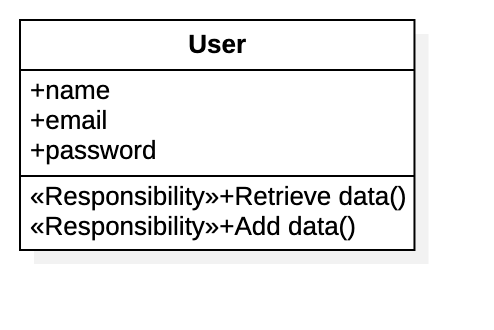
\includegraphics[width=\linewidth]{Immagini/ADC.png}
%\caption{Solution Domain Class}
%\label{fig:ADC}
%\end{minipage}
%\hfill
%\begin{minipage}[c]{0.6\linewidth}
%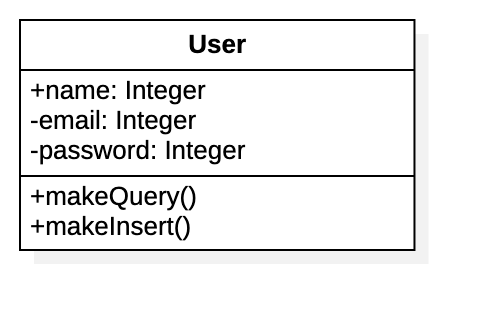
\includegraphics[width=\linewidth]{Immagini/SDC.png}
%\caption{Solution Domain Class}
%\label{fig:SDC}
%\end{minipage}
%\end{figure}	
\newpage
%\item This is the table completed:
\begin{table}[hbt]
\centering
5\begin{tblr}{
  cell{1}{2} = {c=3}{c},
  hlines,
  vlines,
}
                               & \textbf{Developement Phase}                  &                                                &                         \\
\textbf{Aspect}                & \textbf{Analysis}                            & \textbf{Draft}                                 & \textbf{Implementation} \\
\textit{Intended Use}          & to represent the structures in the application domain                              & to provide an overview of the structure of the system                            & implementation of the classes / provide information for the use of the classes         \\
\textit{Terminology}           & that of the problem domain         & that of the solution domain and the problem domain       & that of the solution domain and the problem domain \\
\textit{Class semantics}       & classes are abstractions in the problem domain & classes are abstractions in the solution domain & classes are abstractions in the solution domain \\
\textit{Association semantics} & represents the hierarchy of abstractions in the problem domain & Represents the inheritance of attributes and method by classes & Represents the inheritance of attributes and method by classes \\
\textit{Detail level}          & as high as necessary to model the domain well & low & high \\
\textit{Target group}          & domain experts, developers-analysts & developers-designers & developers, users of the system             
\end{tblr}
\end{table}
	

\end{parlist}
